\subsection{Métodos usados (UP vs. Ágil)}

UP y los métodos ágiles (como Scrum, que usamos para el primer TP) son iterativos incrementales. Sin embargo tienen varias diferencias.

UP se centra en la arquitectura, y facilita su refinamiento progresivo.

En el primer TP teníamos tres artefactos que guíaban el desarrollo de software: un Product Backlog, un Sprint Backlog y un Burndown Chart. Un backlog es simplemente una lista de prioridad de cosas a hacer. El Burndown Chart sirve para graficar el progreso durante la iteración actual. Estas tres herramientas son lo que se usa para planificar y hacer el seguimiento del proyecto en Scrum.

UP, por otro lado, contiene una larga lista de documentos y herramientas para planificar el proyecto. Por ejemplo, una planificación de una iteración de UP es muchísimo más detallada que para Scrum, dado que incluye riesgos, tareas, recursos asignados a tareas y dependencias entre tareas.


\begin{figure}[H]
  \centering
  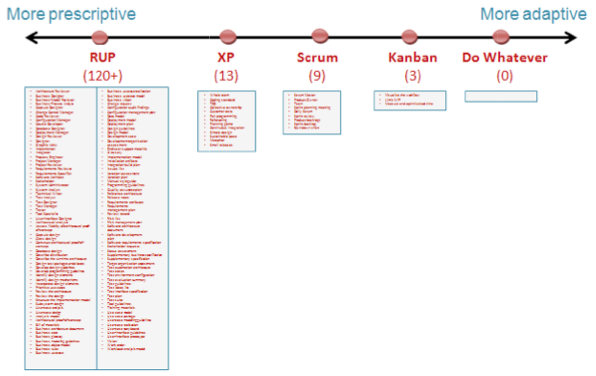
\includegraphics[width=0.7\textwidth]{img/up-agile.png}
  \caption{\normalfont Comparación de varias metodologías de desarrollo.}
\end{figure} 

\subsection{Programming in the small y Programming in the large}

\subsection{Conclusiones generales}
